\documentclass[10pt,draftcls,twocolumn]{IEEEconf}
\usepackage[utf8]{inputenc}
\usepackage{graphicx}


% Title Page
\title{Loss recovery and tail loss performance in Multipath TCP}
\author{KAU}

\begin{document}
\maketitle

\begin{abstract}
\end{abstract}

\section{Introduction}
TCP has two mechanisms for detecting and recovering from packet losses namely Fast Recovery (FR) and Retransmission Timeouts(RTOs). For long flows where there are sufficiently large number of packets 
to be transferred, FR is quicker than RTOs in detecting and recovering packet losses. On the other hand shorter flows which are a majority in the web traffic have to depend on RTOs for packet loss detection 
and recovery thus incurring more latency. A single packet loss in a short flow may take many RTTs to detect and recover. This scenario is also applicable to the packets at the end of the flow (or tail) in a long 
flow.

TCP Loss Probe (TLP)~\cite{ietftlp} a mechanism that allows flows to detect and recover from tail losses much faster than an RTO, thereby speeding up short transfers. With TLP a packet loss in the middle 
of a packet train as well as at the tail end will now trigger the same fast recovery mechanisms. It assumes other algorithms such as early retransmit~\cite{rfc5827} and FACK threshold based recovery are 
present.

In Multi-path-TCP(MPTCP)~\cite{rfc6824}, a connection can have multiple TCP sub flows using different interfaces on different routes. Packet losses in each sub flow are assumed to be detected and recovered 
in a similar fashion as that of TCP. However, It is not completely clear how the loss recovery happens in the implementation and which sub-flow retransmits the lost packets. If the recovery is handled at the 
meta level, the lost packet may be rescheduled and retransmitted at the available sub flow with lowest RTT. If the recovery is handled at the flow level, the packet may be retransmitted in the same sub-flow. 




\section{Related Work}\label{relwork}
TBD.
\section{Scope}\label{scope}

This paper presents the state of the art loss recovery mechanism of MPTCP and presents case for improvement in the tail loss scenario. For understanding the loss recovery and retransmission policies 
in state of the art MPTCP linux implementation version 0.91, we consider specific cases of tail losses.  


\section{Experimental Setup}\label{exsetup}

Experiments use CORE emulation platform with a simple topology as depicted in Figure~\ref{fig1}.
Client is connected to two wireless interfaces 3G/4G and WLAN. Server is connected to a wired router.
Characteristics of the connection setup and assumptions about the parameters are provided in table~\ref{tab1}.
There is no attempt in this study to focus on the effect of link characteristics in retransmission performance.
 
\begin{figure}[!ht]
\begin{center}
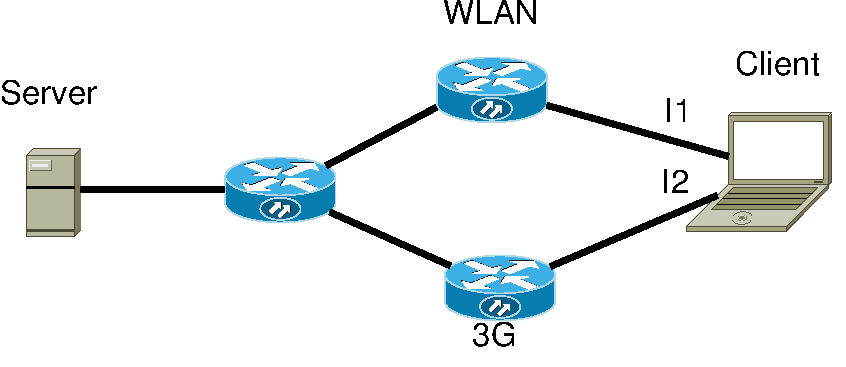
\includegraphics[angle=0, width=0.45\textwidth]{images/fortest.pdf}
\caption{Topology used for Emulation}\label{fig1}
\end{center}
\end{figure}
\begin{center}

\begin{table}
\begin{center}
\begin{tabular}{|c|cccccccccc|}
      \hline
      \multicolumn{1}{c}{} & & \\[\dimexpr-\normalbaselineskip-\arrayrulewidth]
      \textbf{Burst Size} & \multicolumn{10}{c|}{80 Packets} \\
      \hline
      \textbf{Separation Time} & \multicolumn{10}{c|}{2s} \\
      \hline

      \textbf{RTT} & \multicolumn{5}{c|}{20ms-120ms(3G/4G)} & \multicolumn{5}{c|}{20ms-120ms(WLAN)} \\
      \hline 	
      \textbf{Bandwidth} & \multicolumn{5}{c|}{54Mbps(3G/4G)} & \multicolumn{5}{c|}{54Mbps(WLAN)} \\
      \hline
      \textbf{Loss Model} & \multicolumn{10}{c|}{Deterministic}\\
      \hline
\end{tabular}
\caption{Connection parameters}\label{tab1}
\end{center}
\end{table}
\end{center}


\subsection{Testing retransmission with deterministic loss patterns}
In order to understand the retransmission behavior of the Linux MPTCP implementation and to reproduce the observed retransmissions, we use a deterministic drop pattern.
Losses generated by using associating netem with corresponding interfaces and dropping the packets. This process is simplified by using the KAUNetem tool~\cite{Garcia2016}. 
MPTCP connection starts with a single TCP subflow and subsequently, one or more subflows are added following an agreement between client and server on the MPTCP protocol 
support and interface availability. So one has to wait in time and packets for the second subflow establishment to understand the MPTCP retransmissions. We send two bursts of 80 
packets each and drop tail packets on one of the interface. This is to ensure that the necessary and sufficient conditions for probe triggering are met and tail loss probe is generated on that
subflow. Three test cases are evaluated with one packet tail loss, two packet tail loss and  one packet along with probe loss. 

In Linux, TCP retransmission features are controlled by a sysctl setting tcp.early.retrans. It has 5 possible values with ranging from 0 to 4 with 3 being Linux default, enables both
ER and TLP. For this analysis, apart from the default setting, we also consider 0 that diasables both ER and TLP and 2 that enables delayed ER. Disabling ER and TLP gives us the performance
of RTO efficiency. Enabling delayed ER gives us combined performance of RTO and delayed ER and provides the possibility to single out the scenarios where TLP is more effective.
Probe loss should be seen as retransmission loss when tcp.early.retrans is 0 or 2.

In each setting, we calculate burst completion time for two bursts of 80 packets each. The setup has server and client with Linux supporting MPTCP running on them. Client has two wireless 
interfaces with one way delay on each interface ranging from 20ms to 120ms. We consider 5 scenarios with delay pairings 20ms-20ms, 20ms-30ms, 20ms-120ms, 30ms-20ms, 120ms-20ms to understand 
the effect of delay difference in the performance. These scenarios are choosen to evaluate the effect of symmetry, mild asymmetry and higher asymmetry in link delays. 

\section{Observations and Discussion}\label{disc}


\subsection{TCP}
Retransmission behavior of TCP is seen a base case for MPTCP performance as each individual MPTCP subflow is a TCP flow in itself. Our analysis
starts with the results using TCP and compares it with that of the MPTCP. Figures ~\ref{t1p},~\ref{t2p},~\ref{t1pp} represent the comparison of TCP 
burst completion times. Path asymmetry is irrelevant as the TCP uses single path.

In the case of single packet tail loss, there is no difference in burst completion times of ER setting 0,2 and 3. All the cases depend on the RTO
to recover from loss. In two packet tail loss case, ER setting 0 and 2 have similar performance while ER setting 3 improves burst completion time
by using TLP. If the probe or retransmission is lost, then ER 3 still performs better than 0 and 2 as it waits for one RTO and one probe timeout
instead of two RTOs in other two cases.

\begin{figure}[!ht]
\begin{center}
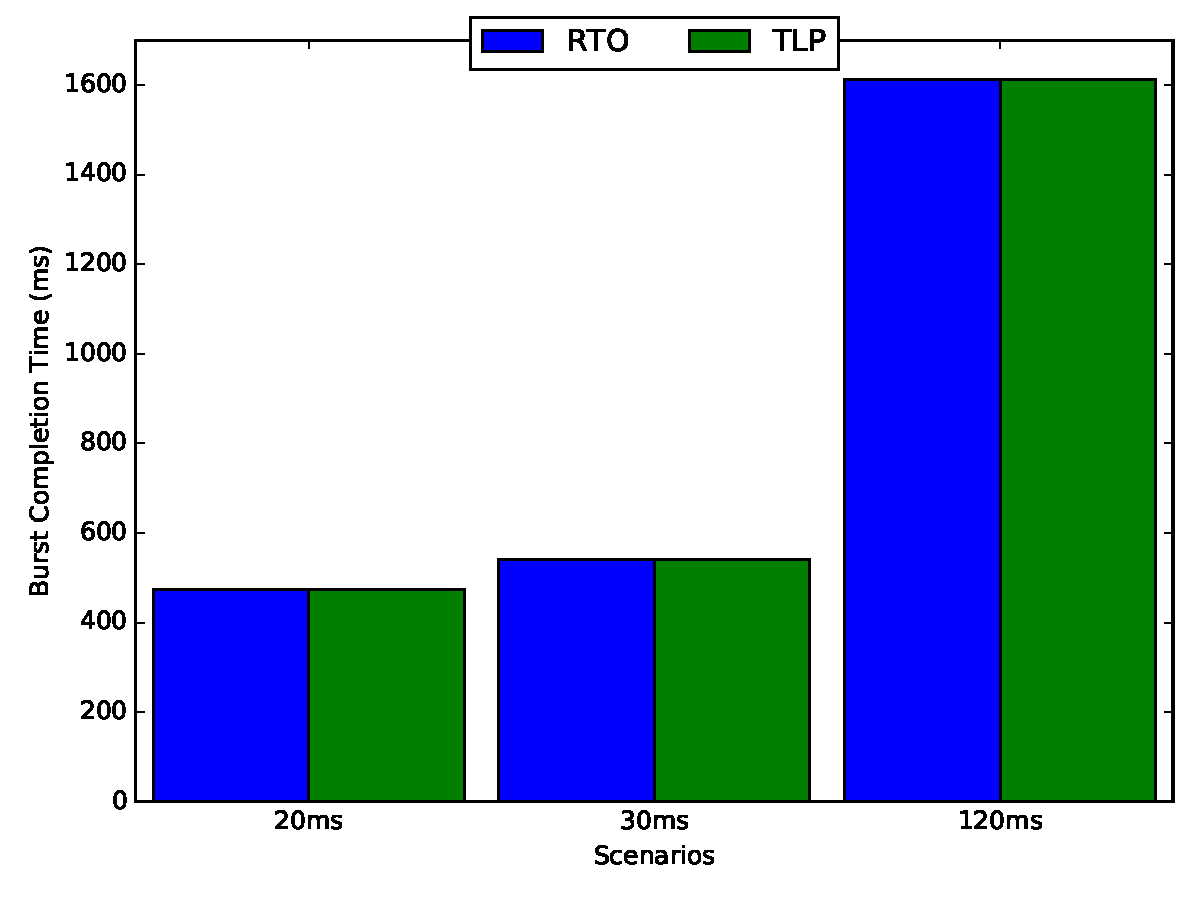
\includegraphics[angle=0, width=0.46\textwidth,natwidth=578.16,natheight=433.62]{plots/T1P.pdf}
\caption{Single packet tail loss using TCP}\label{t1p}
\end{center}
\end{figure}



\begin{figure}[!ht]
\begin{center}
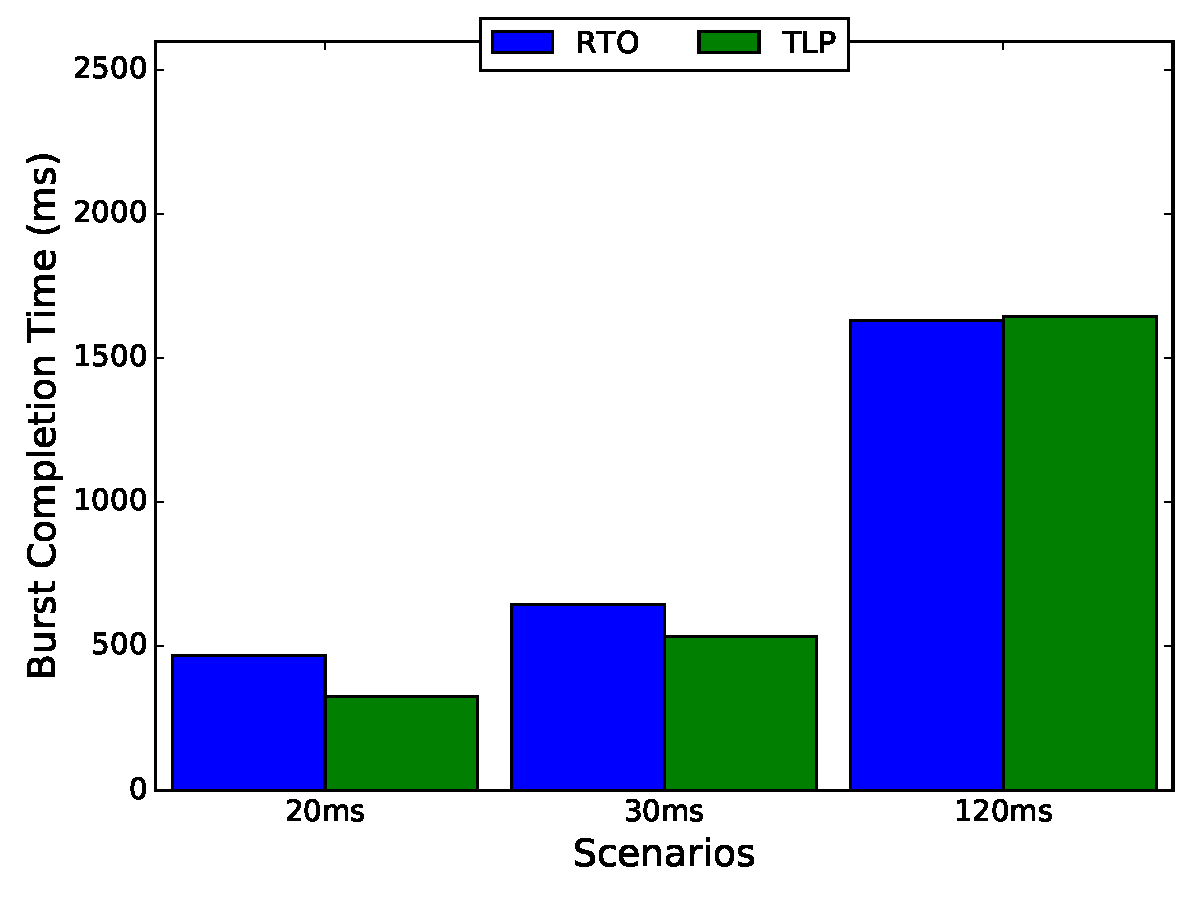
\includegraphics[angle=0, width=0.46\textwidth,natwidth=578.16,natheight=433.62]{plots/T2P.pdf}
\caption{Two packet tail loss using TCP}\label{t2p}
\end{center}
\end{figure}


\begin{figure}[!ht]
\begin{center}
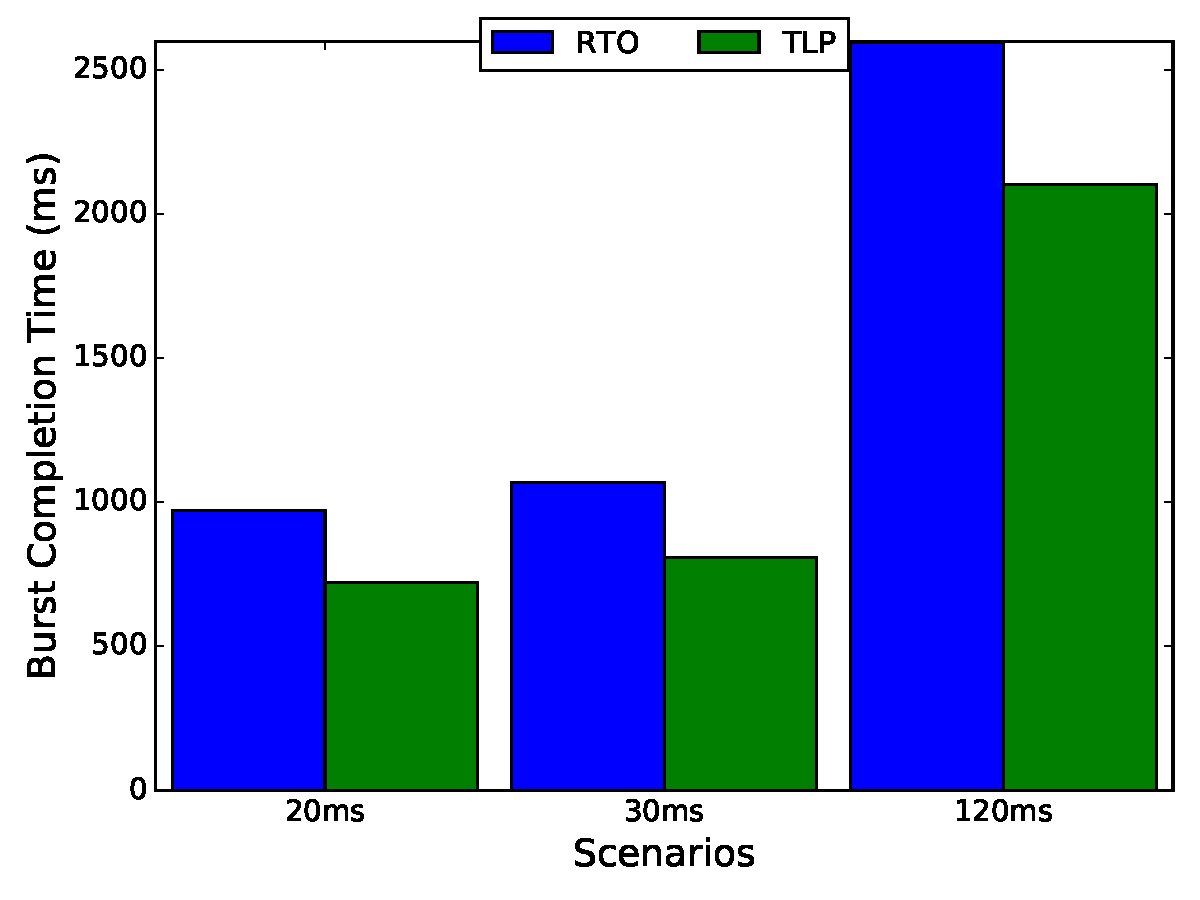
\includegraphics[angle=0, width=0.46\textwidth, natwidth=578.16,natheight=433.62]{plots/T1PP.pdf}
\caption{Single packet tail loss together with probe loss using TCP}\label{t1pp}
\end{center}
\end{figure}

\subsection{MPTCP}


The expected retransmission behavior of MPTCP for different settings of ER is shown 
in~\ref{timing1P},~\ref{timing1PP} and ~\ref{timing2P}.

\begin{figure}[!ht]
\begin{center}
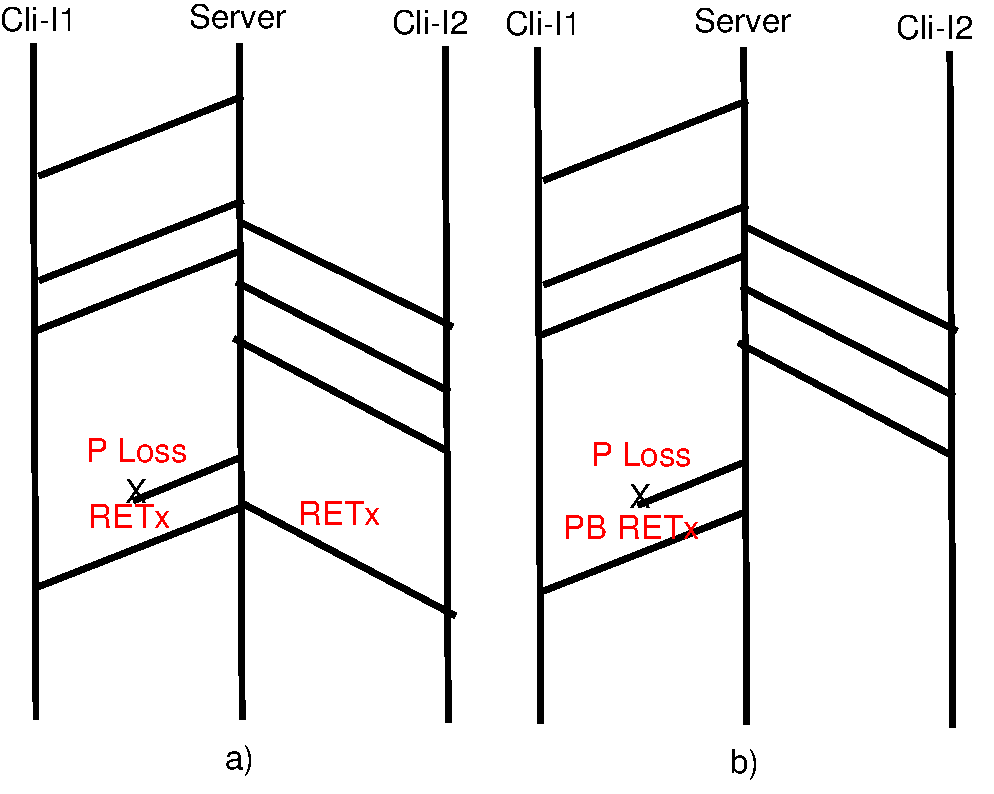
\includegraphics[angle=0, width=0.45\textwidth, natwidth=610, natheight=400]{images/timing1P.pdf}
\end{center}
\caption{Timing diagram of MPTCP behavior with one packet tail loss a) STD b) LIN}\label{timing1P}
\end{figure}

\begin{figure}[!ht]
\begin{center}
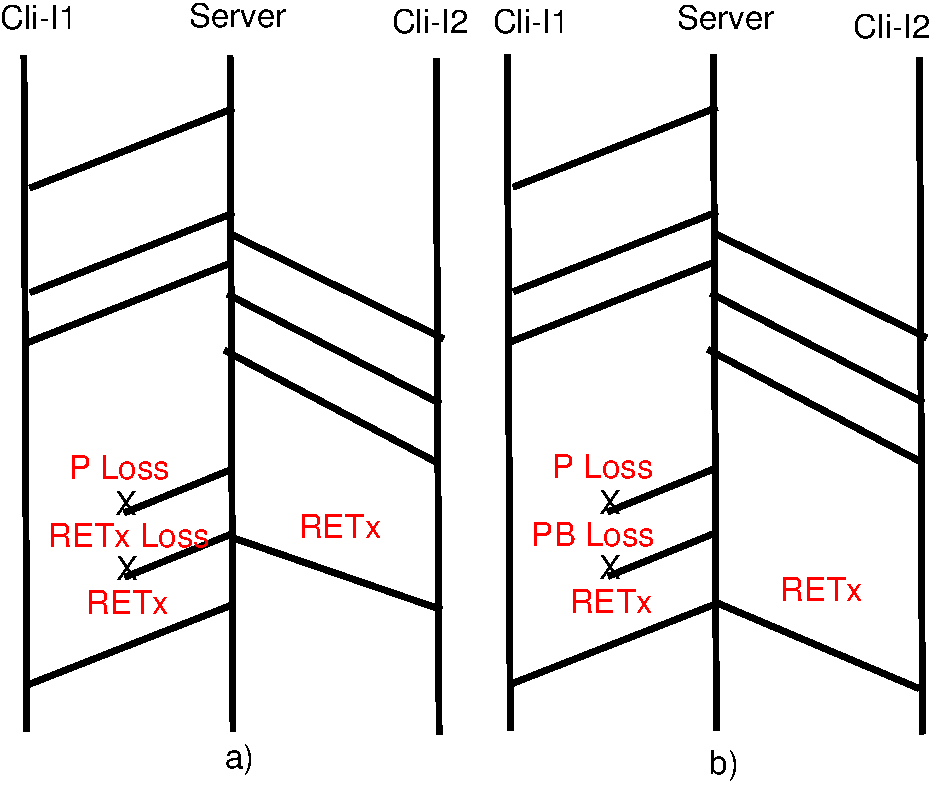
\includegraphics[angle=0, width=0.45\textwidth, natwidth=610, natheight=400]{images/timing1PP.pdf}
\end{center}
\caption{Timing diagram of MPTCP behavior with one packet and next probe loss a) STD b) LIN}\label{timing1PP}
\end{figure}

\begin{figure}[!ht]
\begin{center}
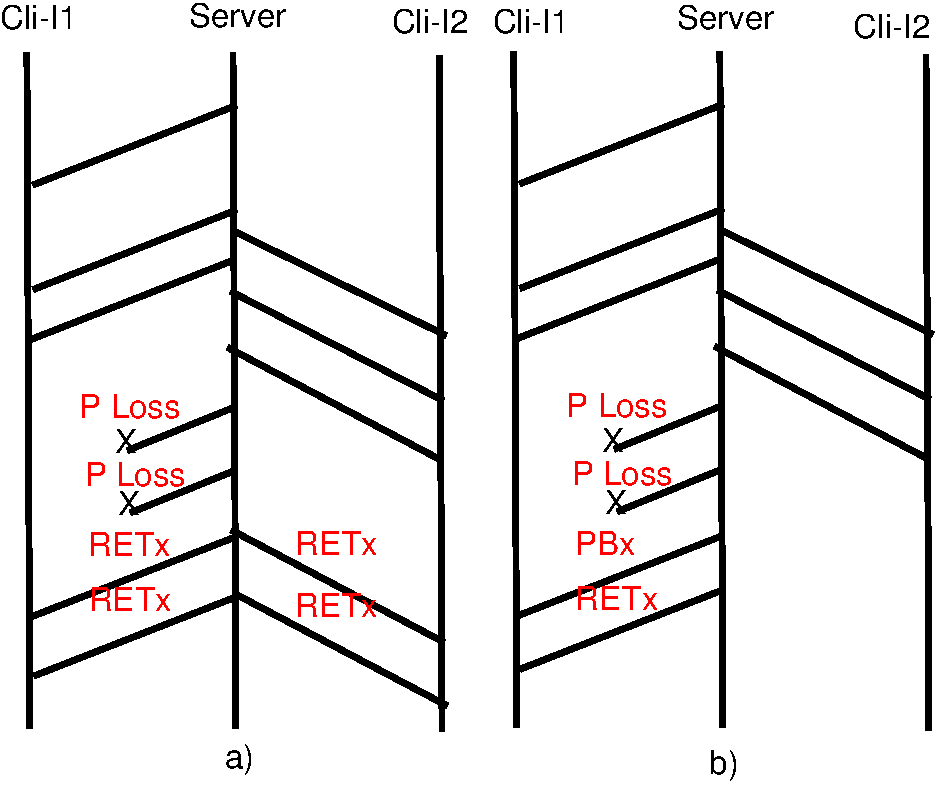
\includegraphics[angle=0, width=0.45\textwidth, natwidth=610, natheight=400]{images/timing2P.pdf}
\end{center}
\caption{Timing diagram of MPTCP behavior with two packet tail loss a) STD b) LIN}\label{timing2P}
\end{figure}



Experiments performed on CORE emulator with the setup mentioned in section\ref{exsetup}.
MPTCP is sensitive to path asymmetry in general due to the default scheduler being shortest RTT based scheduler. Wireshark and tcptrace
analysis provides information on the TCP retransmissions at the subflow level.  


Figure~\ref{1p} provides burst completion time comparison of different ER sysctl settings considered with one packet loss. The results show the improvements
in burst completion time with ER and TLP enabled compared to both disabled only when there is delay difference.

\begin{figure}[!ht]
\begin{center}
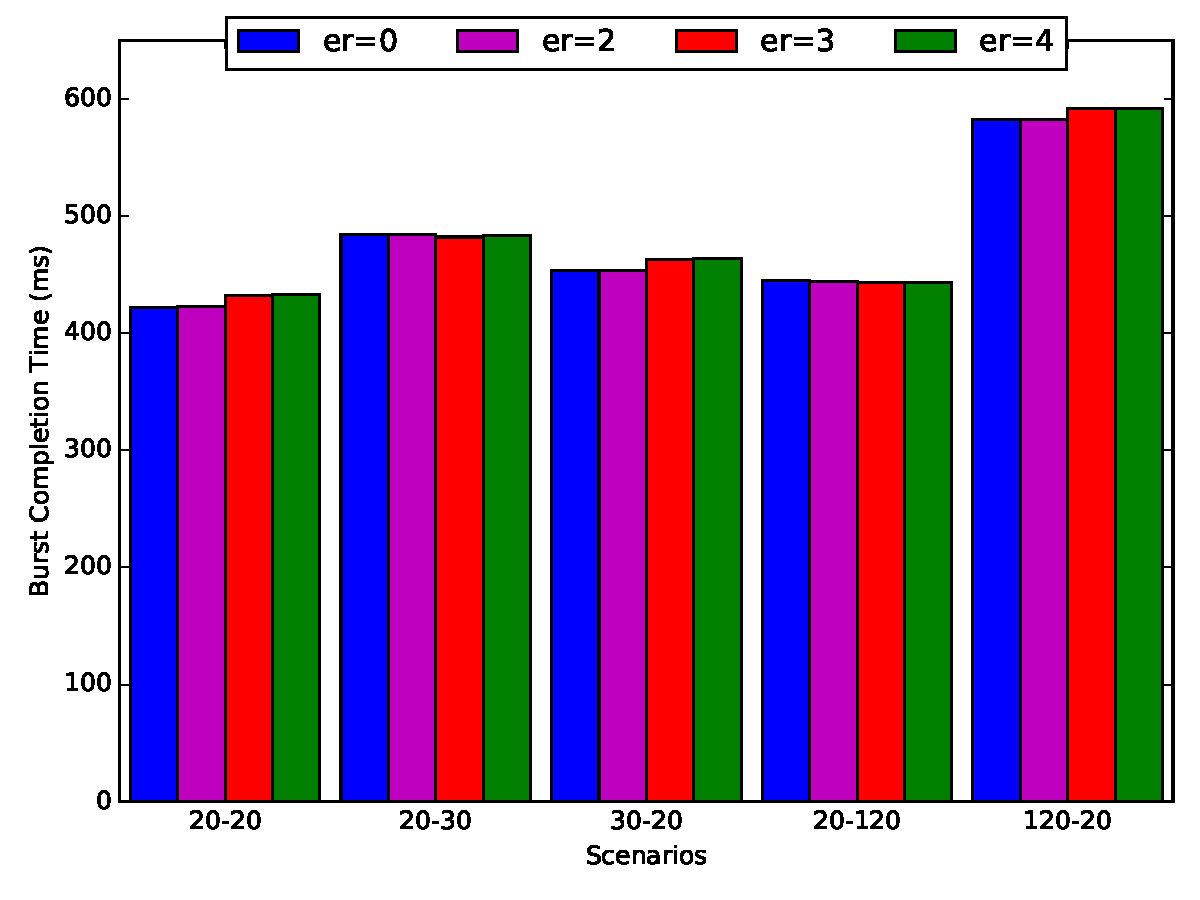
\includegraphics[angle=0, width=0.46\textwidth,natwidth=578.16,natheight=433.62]{plots/1P.pdf}
\caption{Single packet tail loss using MPTCP}\label{1p}
\end{center}
\end{figure}

In packet trace inspection, it is easy to observe the use of TLP with two packet tail loss. The last packet will be retransmitted first in this case.
With one packet tail loss one has to compare the RTT and last packet retransmission time to check the use of TLP.
To further validate the results with one packet tail loss, we consider two packet tail loss and the results are shown in~\ref{2p}.
In this case, ER=3 setting performs better than the other two settings in all scenarios except when the packets lost on high delay interface. 


\begin{figure}[!ht]
\begin{center}
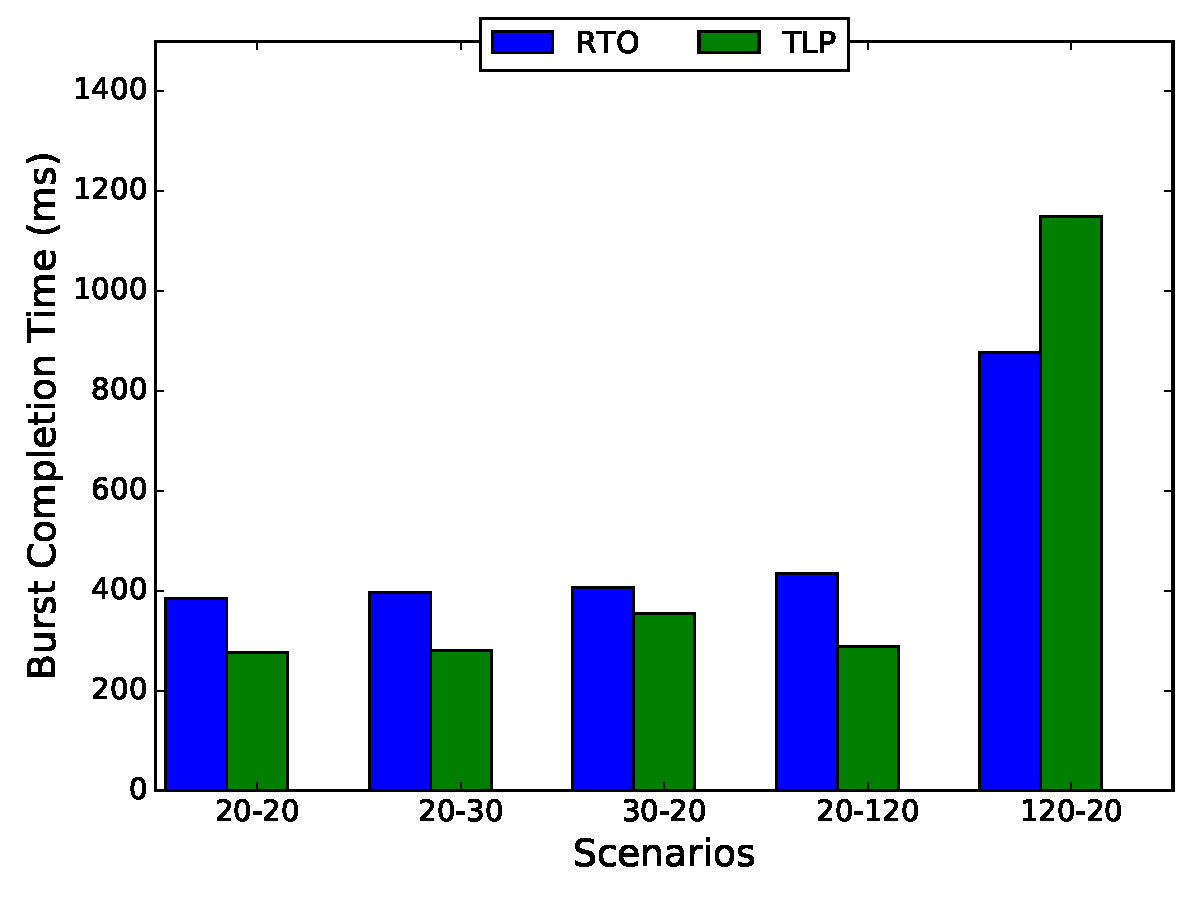
\includegraphics[angle=0, width=0.46\textwidth,natwidth=578.16,natheight=433.62]{plots/2P.pdf}
\caption{Two packet tail loss using MPTCP}\label{2p}
\end{center}
\end{figure}

To further study the performance of TLP in improving latency, we tried to drop the probe packet along with the last packet. In this case ER=0
setting results much lower burst completion times. Use of TLP did not improve the burst completion time as we saw in TCP for ER=3. The reason
lies in the way the retransmission and loss probe transmission carried out in MPTCP. Retransmission occurs after an RTO time on both paths.
Even if retransmission fails on one path, the client receives the packet on the other path as shown in Fig~\ref{timing1P}. For TLP, in
current implementation, the loss probe sent on the actual path of first transmission but not on both paths. This incorrect impartation of
TLP from TCP to MPTCP led to the increase burst completion time by an RTO for MPTCP. 


\begin{figure}[!ht]
\begin{center}
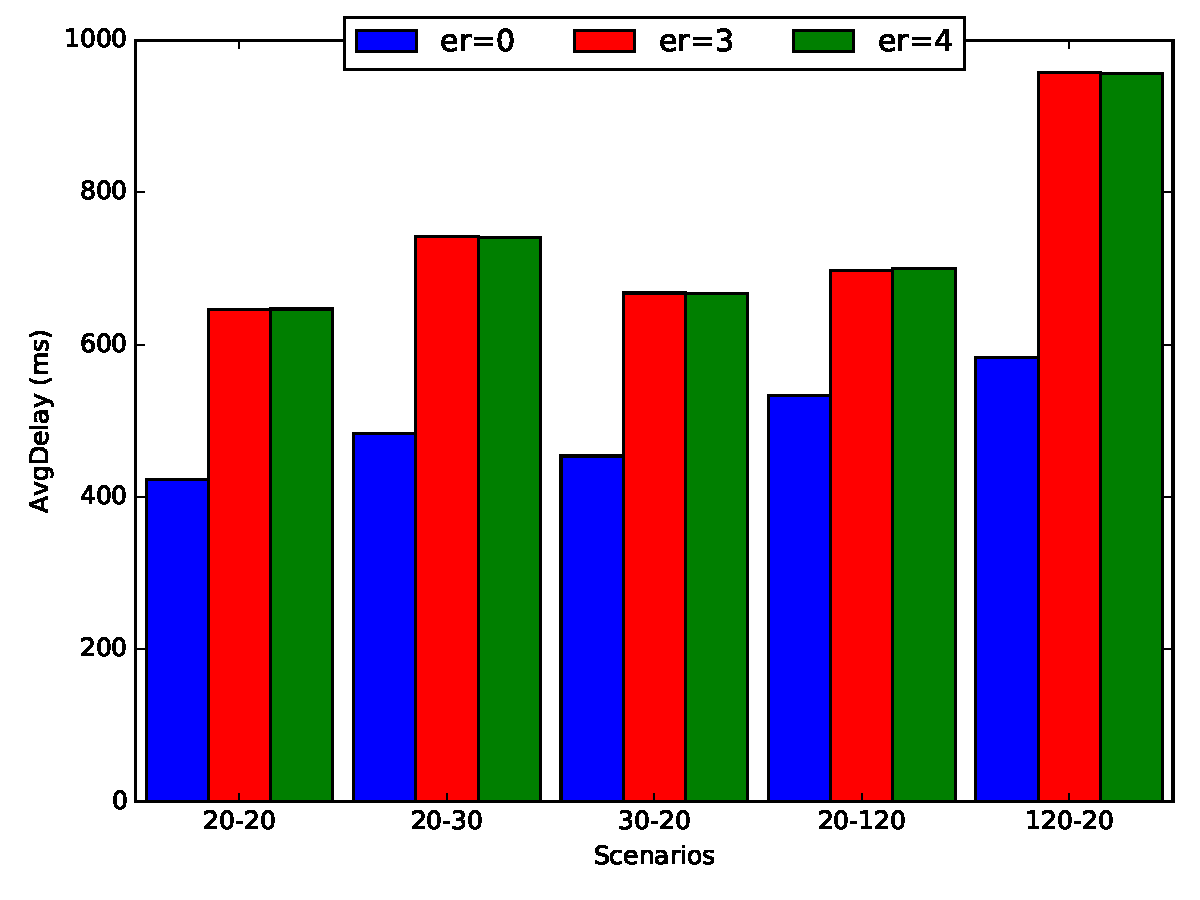
\includegraphics[angle=0, width=0.46\textwidth, natwidth=578.16,natheight=433.62]{plots/1PP.pdf}
\caption{Single packet tail loss together with probe loss using MPTCP}\label{1pp}
\end{center}
\end{figure}





%\begin{table}[!ht]
%\centering
%\caption{Tail loss scenarios with tcp.early.retrans = 3 default}
%\label{ret3}
%\begin{tabular}{|l|l|l|l|l|}
%\hline
% testcase   & Asymmetry   & Metalevel          & Subflowlevel       &  \\\hline
%Tail drop 1 & 20ms - 30ms & rexmt in same path & rexmt in same path &  \\\hline
%Tail drop 2 & 30ms - 20ms & rexmt in same path & TBC                &  \\\hline
%Tail drop 3 & 20ms - 20ms & rexmt in same path & TBC                &  \\ \hline
%\end{tabular}
%\end{table}





%\begin{table}[!ht]
%\centering
%\caption{Tail loss scenarios with tcp.early.retrans = 0 ER disabled}
%\label{ret0}
%\begin{tabular}{|l|l|l|l|l|}
%\hline
% testcase   & Asymmetry   & Metalevel          & Subflowlevel       &  \\\hline
%Tail drop 1 & 20ms - 30ms & rexmt in same path & rexmt in same path &  \\\hline
%Tail drop 2 & 30ms - 20ms & rexmt in same path & TBC                &  \\\hline
%Tail drop 3 & 20ms - 20ms & rexmt in same path & TBC                & \\ \hline
%Tail drop 4 & 20ms - 120ms &  			&		&  \\ \hline
%Tail drop 5 & 120ms - 20ms &  			& 		& \\ \hline 
%\end{tabular}
%\end{table}


%\begin{table}[!ht]
%\centering
%\caption{Tail loss scenarios with tcp.early.retrans = 4 TLP disabled}
%\label{ret4}
%\begin{tabular}{|l|l|l|l|l|}
%\hline
% testcase   & Asymmetry   & Metalevel          & Subflowlevel       &  \\\hline
%Tail drop 1 & 20ms - 30ms & rexmt in same path & rexmt in same path &  \\\hline
%Tail drop 2 & 30ms - 20ms & rexmt in same path & TBC                &  \\\hline
%Tail drop 3 & 20ms - 20ms & rexmt in same path & TBC                & \\ \hline
%\end{tabular}
%\end{table}


\section{Improvments to TLP for MPTCP}
The goal of Tail Loss Probe(TLP) is to reduce tail latency of short flows. It achieves this by converting retransmission timeouts (RTOs) occuring due to tail losses (losses at end of transactions) into fast recovery. TLP transmits one packet in two round-trips when a connection is in Open state and isn't receiving any ACKs. The transmitted packet, aka loss probe, can be either new or a retransmission. When there is tail loss, the ACK from a loss probe triggers FACK/early-retransmit based fast recovery, thus avoiding a costly retransmission timeout. Our results show that current TLP implementation does not improve the performance in MPTCP and incur more latency.

Current implementation of TLP is at the TCP flow level. In the event of RTO timeout the MPTCP retransmission happens with a reinjection in to scheduler along with sending lost packet on the same path. But in the Event of Probe timeout, the loss probe packet is being sent on the same path without injecting in to scheduler.  Modifications should reinject the probe packet in to the mptcp scheduler in the event of PTO.

\subsection{Example scenario where MPTCP TLP could incur more latency}

Use a traffic pattern where there is new burst to send before the RTO after a tail loss triggering TLP on a flow.


\section{Evaluation of proposal}

Initial testing with customized program to send bursts of packets with fixed burst seperation. Adjust the burst seperation to get the desired scenario.
Results comparing the MPTCP-TLP for the considered cases are provided in figures~\ref{1pn},~\ref{2pn} and ~\ref{1ppn}. The improvement in latency
performance is seen Single packet tail loss with probe loss scenario. Single packet loss and Two packet loss scenarios provide increase in latency.
Analysis required in these two cases.


\begin{figure}[!ht]
\begin{center}
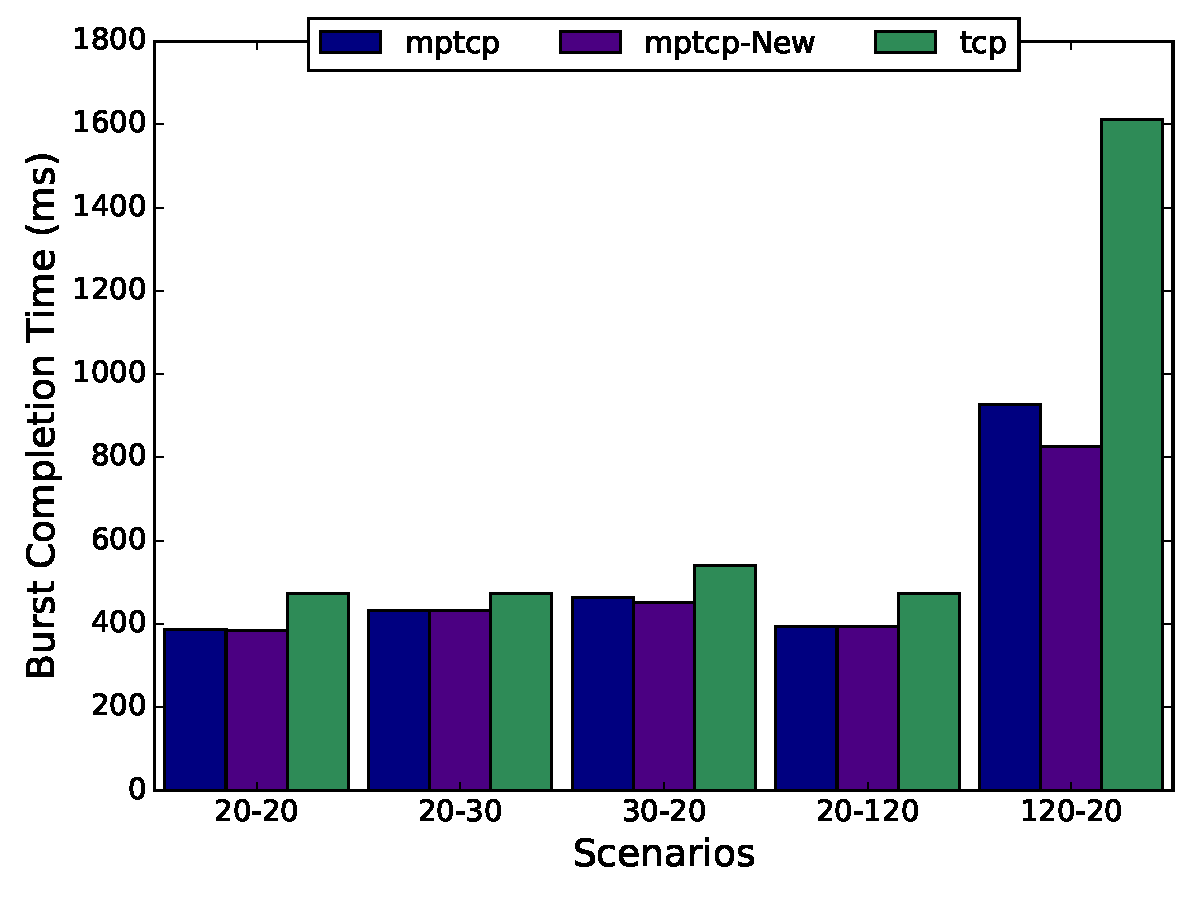
\includegraphics[angle=0, width=0.46\textwidth, natwidth=578.16,natheight=433.62]{plots/1PNew.pdf}
\caption{Single packet tail loss comparision with MPTCP-TLP}\label{1pn}
\end{center}
\end{figure}

\begin{figure}[!ht]
\begin{center}
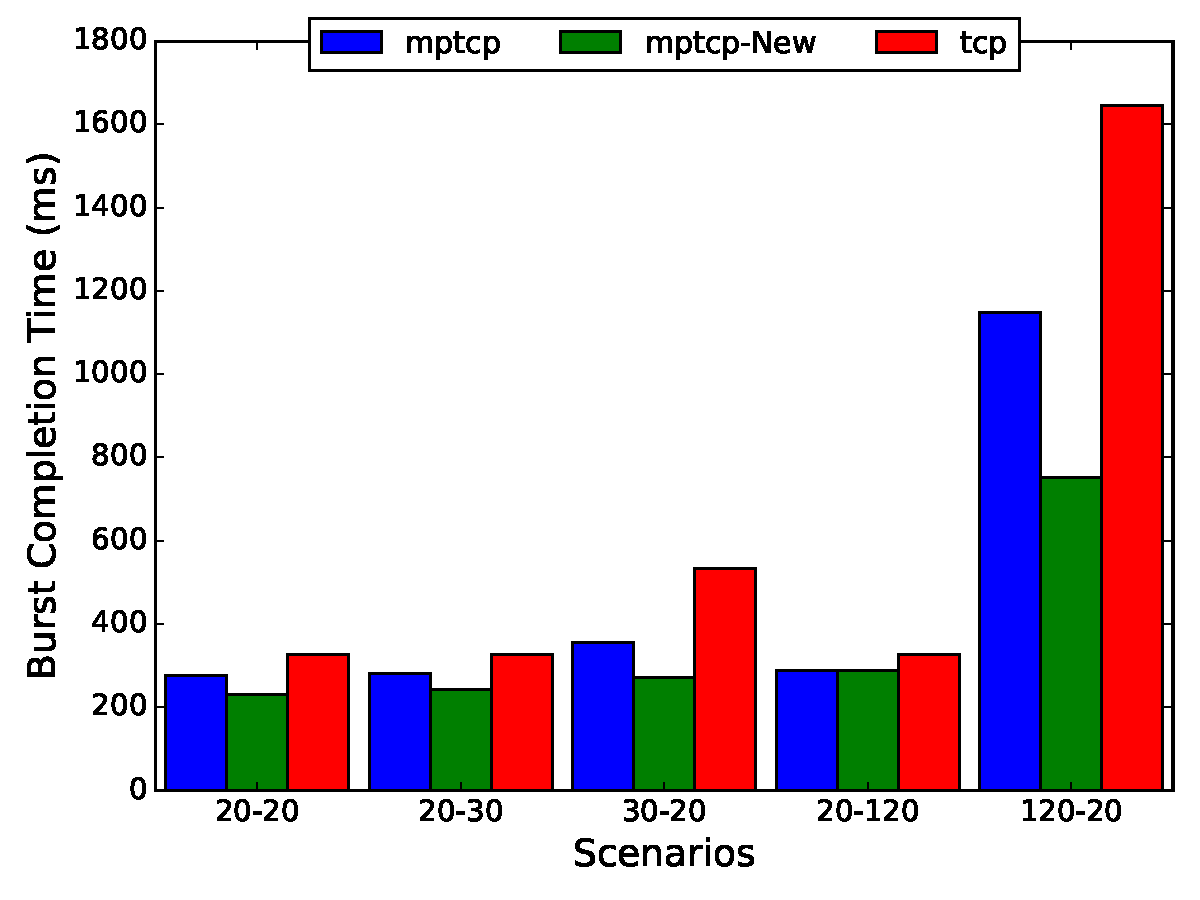
\includegraphics[angle=0, width=0.46\textwidth, natwidth=578.16,natheight=433.62]{plots/2PNew.pdf}
\caption{Two packet tail loss comparison with MPTCP-TLP}\label{2pn}
\end{center}
\end{figure}

\begin{figure}[!ht]
\begin{center}
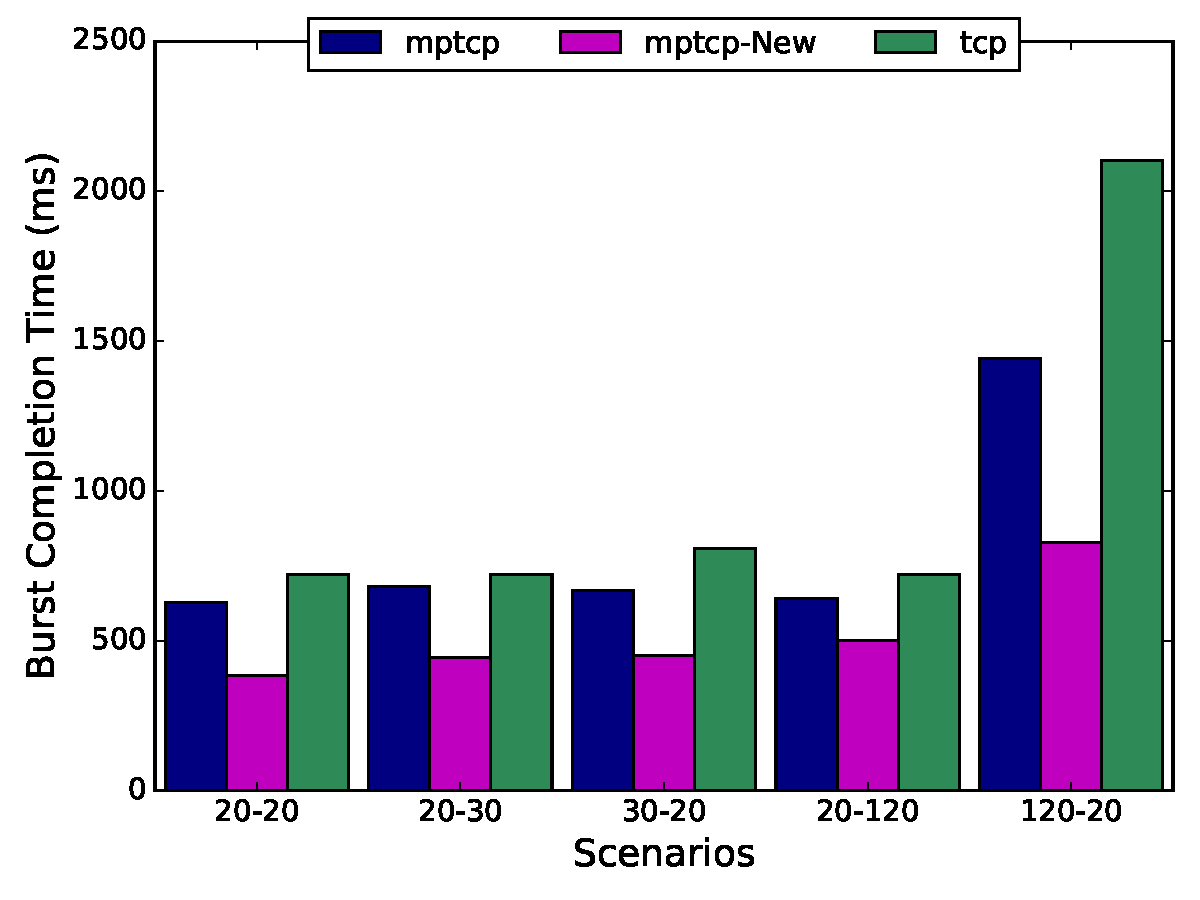
\includegraphics[angle=0, width=0.46\textwidth, natwidth=578.16,natheight=433.62]{plots/1PPNew.pdf}
\caption{Single packet tail loss together with probe loss with MPTCP-TLP}\label{1ppn}
\end{center}
\end{figure}




\bibliographystyle{IEEEtran}
\bibliography{mptcp-retrans}
\end{document} 
